% =====================================================================
% Rapport d'avancement Sprint 4 - SkillSeek AI
% Auteur : Aymen Benrbib - ESI (ISITD) - Stage BC SKILLS 2026
% Compilation : pdflatex (Overleaf : compiler "pdfLaTeX", 2 passes)
% Ressources attendues a cote du .tex :
%   - bc_skills.jpg          (logo de l'entreprise)
%   - captures/*.jpg         (captures d'ecran de la plateforme)
% =====================================================================
\documentclass[11pt,a4paper]{article}

\usepackage[utf8]{inputenc}
\usepackage[T1]{fontenc}
\IfFileExists{french.ldf}{%
  \usepackage[french]{babel}%
}{%
  \renewcommand{\contentsname}{Table des matières}%
  \renewcommand{\figurename}{Figure}%
  \renewcommand{\tablename}{Tableau}%
}
\usepackage{lmodern}
\usepackage[margin=2.4cm]{geometry}
\usepackage{graphicx}
\usepackage{xcolor}
\usepackage{booktabs}
\usepackage{array}
\usepackage{longtable}
\usepackage{enumitem}
\usepackage{titlesec}
\usepackage{fancyhdr}
\usepackage{tikz}
\usepackage{float}
\usepackage{listings}
\usepackage{caption}
\usetikzlibrary{arrows.meta, positioning, shapes.geometric, fit, backgrounds, patterns}
\usepackage{hyperref}

\raggedbottom

% ------------------ Couleurs ------------------
\definecolor{primaire}{HTML}{1F3A5F}
\definecolor{accent}{HTML}{2E86AB}
\definecolor{fondclair}{HTML}{EEF4F8}
\definecolor{vert}{HTML}{2E7D5B}
\definecolor{gris}{HTML}{6B7A8F}
\definecolor{grisclair}{HTML}{C9D3DD}
\definecolor{ambre}{HTML}{B5820A}

\hypersetup{colorlinks=true, linkcolor=primaire, urlcolor=accent,
  pdftitle={Rapport d'avancement Sprint 4 - SkillSeek AI}, pdfauthor={Aymen Benrbib}}

% ------------------ Titres ------------------
\titleformat{\section}{\Large\bfseries\color{primaire}}{\thesection}{0.6em}{}
\titlespacing*{\section}{0pt}{14pt}{8pt}
\titleformat{\subsection}{\large\bfseries\color{primaire}}{\thesubsection}{0.6em}{}
\titleformat{\subsubsection}{\normalsize\bfseries\color{accent}}{\thesubsubsection}{0.6em}{}

\captionsetup{font=small, labelfont={bf, color=primaire}}

% ------------------ En-tete / pied ------------------
\pagestyle{fancy}
\fancyhf{}
\fancyhead[L]{\small\color{primaire} Rapport d'avancement Sprint 4 -- SkillSeek AI}
\fancyhead[R]{\small\color{primaire} BC SKILLS -- 2026}
\fancyfoot[C]{\small\thepage}
\renewcommand{\headrulewidth}{0.4pt}

% ------------------ Styles TikZ ------------------
\tikzset{
  bloc/.style={rectangle, rounded corners=2pt, draw=primaire, fill=fondclair,
    text=primaire, font=\small\bfseries, minimum height=9mm,
    minimum width=24mm, align=center, inner sep=1.8mm},
  blocia/.style={bloc, draw=accent, fill=white, text=accent},
  blocneuf/.style={bloc, draw=vert, fill=white, text=vert},
  fleche/.style={-{Stealth[length=2.2mm]}, thick, color=primaire},
  flechefine/.style={-{Stealth[length=1.8mm]}, color=gris},
  etiquette/.style={font=\scriptsize, color=primaire, align=center},
}

\lstset{
  basicstyle=\ttfamily\scriptsize,
  backgroundcolor=\color{fondclair},
  frame=single,
  rulecolor=\color{gris},
  breaklines=true,
  keywordstyle=\color{primaire}\bfseries,
  commentstyle=\color{vert},
  showstringspaces=false,
  language=Python
}

% ------------------ Insertion d'une capture ------------------
% \capture{fichier}{legende}{label}
\newcommand{\capture}[3]{%
  \begin{figure}[H]
    \centering
    \IfFileExists{captures/#1.jpg}{%
      \fbox{\includegraphics[width=0.96\textwidth]{captures/#1}}%
    }{%
      \fbox{\parbox[c][4cm][c]{0.9\textwidth}{\centering\color{gris}%
        Capture manquante : \texttt{\detokenize{captures/#1.jpg}}}}%
    }
    \caption{#2}
    \label{#3}
  \end{figure}%
}

\begin{document}

% =====================================================================
% PAGE DE GARDE
% =====================================================================
\begin{titlepage}
  \centering
  \IfFileExists{bc_skills.jpg}{%
    
\includegraphics[width=4.5cm]{bc_skills.jpg}%
  }{%
    \fbox{\parbox[c][3cm][c]{4.5cm}{\centering\small\color{gris}
      Logo BC SKILLS\\ (ajouter \texttt{bc\_skills.jpg})}}%
  }\\[1cm]
  {\color{primaire}\rule{\textwidth}{2pt}}\\[1cm]
  {\large École des Sciences de l'Information (ESI)}\\[0.2cm]
  {\normalsize Filière : Ingénierie des Systèmes d'Information et Transformation Digitale (ISITD)}\\[2cm]

  {\Huge\bfseries\color{primaire} Rapport d'avancement}\\[0.4cm]
  {\Large\bfseries\color{accent} Sprint 4}\\[0.7cm]
  {\LARGE\bfseries SkillSeek AI}\\[0.8cm]
  {\large Plateforme intelligente de gestion du recrutement\\
   Apprentissage supervisé et évaluation des performances}\\[2.5cm]

  \begin{tabular}{ll}
    \textbf{Auteur :}              & Aymen Benrbib \\[2mm]
    \textbf{Organisme d'accueil :} & BC SKILLS \\
  \end{tabular}\\[2.5cm]

  {\color{primaire}\rule{\textwidth}{2pt}}
\end{titlepage}

\tableofcontents
\newpage

% =====================================================================
\section{Objet du rapport}
% =====================================================================
Ce document clôt le \textbf{Sprint~4}, dernier sprint du stage, et constitue à ce titre le dernier rapport d'avancement du projet \textbf{SkillSeek AI}. Il rend compte de deux périodes de nature différente.

La première (07/08 -- 10/08) porte sur le fait marquant du sprint : la \textbf{reprise de l'apprentissage supervisé}, écarté au Sprint~3 faute de corpus, désormais réalisé, évalué et intégré. Une place importante y est donnée à la méthode d'évaluation, car un modèle d'apprentissage se juge moins à la performance qu'il affiche qu'au protocole qui l'établit : ce rapport expose les quatre protocoles appliqués, les deux erreurs de mesure qu'ils ont permis de détecter, et le chiffre finalement retenu --- modeste et vérifié plutôt que flatteur et fragile.

La seconde (11/08 -- 16/08) porte sur le passage de la plateforme d'un prototype fonctionnel à un \textbf{produit exploitable} : consolidation du cloisonnement entre recruteurs, instrumentation de la chaîne d'analyse, restitution décisionnelle intégrée à l'application, orientation du candidat, et industrialisation de la construction et de la livraison. Cette seconde partie ne figurait pas intégralement au périmètre initial ; la section~\ref{sec:consolidation} expose ce qui l'a motivée.

% =====================================================================
\section{Rappel des sprints précédents}
% =====================================================================
Le \textbf{Sprint~1} (06/07 -- 15/07) a livré le socle technique : environnement conteneurisé, intégration continue, modèle de données, authentification par jeton et contrôle d'accès par rôles appliqué en temps réel.

Le \textbf{Sprint~2} (16/07 -- 27/07) a livré l'interface complète — dix-huit écrans répartis entre les trois profils d'utilisateurs — les parcours métier de bout en bout et les notifications événementielles.

Le \textbf{Sprint~3} (28/07 -- 06/08) a livré le cœur analytique : lecture des documents avec reconnaissance optique en repli, reconstitution d'un profil structuré selon les conventions professionnelles d'analyse de curriculum vitæ, moteur de règles à critères éliminatoires tracés, proximité sémantique multilingue, et assistant conversationnel fondé sur les données réelles de la plateforme.

\medskip
\noindent\textbf{Point de départ du Sprint~4.} Le rapport du Sprint~3 actait le renoncement à l'apprentissage supervisé, motivé par l'absence de corpus étiqueté disponible. Cette décision a été révisée au début du présent sprint ; la section~\ref{sec:revision} en expose les raisons et les conséquences.

% =====================================================================
\section{Synthèse de l'avancement}
% =====================================================================

\subsection{État global}

\begin{center}
\small
\begin{tabular}{lccp{5.4cm}}
  \toprule
  \textbf{Sprint} & \textbf{Période} & \textbf{État} & \textbf{Périmètre} \\
  \midrule
  Sprint 1 & 06/07 -- 15/07 & \textcolor{vert}{\textbf{Terminé}} & Socle technique, base de données, sécurité \\[1mm]
  Sprint 2 & 16/07 -- 27/07 & \textcolor{vert}{\textbf{Terminé}} & Interface, parcours métier, notifications \\[1mm]
  Sprint 3 & 28/07 -- 06/08 & \textcolor{vert}{\textbf{Terminé}} & Analyse des CV, classement explicable \\[1mm]
  Sprint 4 & 07/08 -- 16/08 & \textcolor{vert}{\textbf{Terminé}} & Apprentissage supervisé, consolidation, industrialisation \\
  \bottomrule
\end{tabular}
\end{center}

\vspace{2mm}
\noindent \textbf{La totalité du périmètre fonctionnel du cahier des charges est réalisée}, module d'apprentissage compris. Ce qui subsiste relève des perspectives d'industrialisation --- déploiement effectif sur un serveur, tests de bout en bout, métrologie d'exploitation --- et non de fonctions promises non livrées ; la section~\ref{sec:perspectives} le détaille sans le minimiser.

\subsection{Tâches du Sprint 4}

\begin{center}
\small
\begin{tabular}{clp{6.4cm}c}
  \toprule
  \textbf{ID} & \textbf{Tâche} & \textbf{Livrable vérifié} & \textbf{État} \\
  \midrule
  S3-04 & Corpus d'apprentissage & 8\,000 appariements étiquetés, exploitables après contrôle & \textcolor{vert}{OK} \\
  S3-06 & Modèle supervisé & Classifieur binaire, 17 indicateurs, évalué sous 4 protocoles & \textcolor{vert}{OK} \\
  S4-01 & Intégration au score & Ajustement borné, règles métiers souveraines & \textcolor{vert}{OK} \\
  S4-02 & Robustesse du dispositif & Fonctionnement garanti en l'absence de modèle & \textcolor{vert}{OK} \\
  S3-07 & Audit de biais & Écart mesuré sur attributs non pertinents & \textcolor{vert}{OK} \\
  S4-03 & Décisionnel & Écran d'analyse intégré et vues destinées à Power BI & \textcolor{vert}{OK} \\
  S4-04 & Indicateurs du cahier des charges & Mesure du dispositif complet, protocole explicité & \textcolor{vert}{OK} \\
  S4-07 & Documentation et soutenance & Guides d'exploitation, script d'enregistrement & \textcolor{vert}{OK} \\
  \midrule
  \multicolumn{4}{l}{\textit{Hors périmètre initial, engagés en seconde partie de sprint}} \\[1mm]
  S4-08 & Cloisonnement par périmètre & Accès aux ressources vérifié route par route & \textcolor{vert}{OK} \\
  S4-09 & Orientation du candidat & Classement des offres à partir du profil déclaré & \textcolor{vert}{OK} \\
  S4-10 & Observabilité & Chronométrage par étape, provenance, sondes & \textcolor{vert}{OK} \\
  S4-11 & Industrialisation & Six travaux d'intégration, images publiées, veille & \textcolor{vert}{OK} \\
  \midrule
  S4-05 & Tests de bout en bout & Parcours automatisés en navigateur & \textcolor{ambre}{Non réalisé} \\
  S4-12 & Déploiement sur serveur & Procédure écrite, non activée & \textcolor{ambre}{Non réalisé} \\
  \bottomrule
\end{tabular}
\end{center}

\vspace{2mm}
\noindent Les tâches S3-04 et S3-06, déclarées écartées au Sprint~3, ont été réintégrées et achevées. La tâche S4-01 ne figurait pas au périmètre initial : elle est la conséquence directe de cette réintégration. Les tâches S4-08 à S4-11 procèdent d'une relecture critique du code menée après l'intégration du modèle, exposée en section~\ref{sec:consolidation}. Les deux tâches non réalisées sont assumées et justifiées en section~\ref{sec:perspectives}.

\subsection{Indicateurs de réalisation}

\begin{center}
\small
\begin{tabular}{lcc}
  \toprule
  \textbf{Indicateur} & \textbf{Sprint 3} & \textbf{Fin de Sprint 4} \\
  \midrule
  Écrans livrés & 18 & \textbf{22} \\
  Points d'accès de l'interface de programmation & 38 & \textbf{61} \\
  Tests automatisés réussis & 69 & \textbf{192} \\
  Analyse statique du code & sans anomalie & sans anomalie \\
  Appariements du corpus d'apprentissage & — & \textbf{8\,000} \\
  Indicateurs calculés par appariement & — & \textbf{17} \\
  Travaux d'intégration continue & 2 & \textbf{7} \\
  Migrations de schéma & 8 & \textbf{11} \\
  Durée d'analyse d'un curriculum vitæ & $<$ 3 s & $<$ 3 s \\
  \bottomrule
\end{tabular}
\end{center}

\vspace{1mm}
\noindent L'ajout du modèle n'a pas dégradé le temps de traitement : la prédiction s'appuie sur des indicateurs déjà calculés par la chaîne d'analyse existante, et le modèle n'est chargé qu'une seule fois au démarrage du service. Les écrans ajoutés sont l'analyse décisionnelle et l'orientation du candidat, l'un et l'autre décrits en section~\ref{sec:restitution}.

% =====================================================================
\section{Reprise de l'apprentissage supervisé}\label{sec:revision}
% =====================================================================

\subsection{Motif de la révision}
Le renoncement acté au Sprint~3 reposait sur un constat : aucun corpus de curriculum vitæ étiquetés n'avait été identifié, et sa constitution manuelle représentait plusieurs jours de travail au résultat incertain.

Sur indication de l'encadrement, la recherche a été reprise sur les plateformes publiques de partage de jeux de données. Un corpus d'appariements entre curriculum vitæ et descriptions de poste, chaque paire portant un jugement d'adéquation, y a été identifié. La condition qui fondait le renoncement n'était donc plus vérifiée, et la décision a été révisée.

Deux corpus candidats ont d'abord été écartés après contrôle : le premier ne présentait aucun signal exploitable, un modèle entraîné dessus faisant moins bien que la simple prédiction de la classe majoritaire ; le second décrivait des décisions postérieures à l'entretien, information dont un système de présélection ne dispose pas au moment où il opère. Ce contrôle préalable de la pertinence du corpus est une étape à part entière : un modèle appris sur des données qui ne correspondent pas à l'usage visé produit des résultats sans valeur, quelle que soit sa performance apparente.

\subsection{Le corpus retenu}

\begin{center}
\small
\begin{tabular}{lc}
  \toprule
  \textbf{Caractéristique} & \textbf{Valeur} \\
  \midrule
  Appariements (curriculum vitæ, offre) étiquetés & 8\,000 \\
  Curriculum vitæ distincts & 643 \\
  Offres distinctes & 351 \\
  Proportion de profils jugés convenables & 49,6 \% \\
  Langue des documents & anglais \\
  \bottomrule
\end{tabular}
\end{center}

\vspace{2mm}
\noindent Un \textbf{jeu de validation francophone} distinct a par ailleurs été constitué pour ce projet : quatre offres et douze curriculum vitæ rédigés en français, formant vingt-quatre appariements. Il n'intervient jamais dans l'apprentissage et sert exclusivement à vérifier que le modèle, appris sur des documents anglais, reste opérant sur des documents français.

\subsection{Ce que le modèle observe}
Le modèle ne reçoit pas les textes bruts mais dix-sept indicateurs calculés pour chaque paire. Le principe de conception retenu est que \textbf{tous les indicateurs sont relationnels} : chacun décrit un rapport entre le profil et l'exigence, jamais une propriété absolue du document.

\begin{center}
\small
\begin{tabular}{lcp{7.4cm}}
  \toprule
  \textbf{Famille} & \textbf{Nombre} & \textbf{Contenu} \\
  \midrule
  Proximité de sens & 3 & Similarité globale, similarité des compétences, similarité des intitulés de poste \\[1mm]
  Adéquation des compétences & 5 & Part des exigences satisfaites, recouvrement, nombre de compétences communes, exigences manquantes, part du profil utile à l'offre \\[1mm]
  Adéquation de l'expérience & 3 & Rapport, écart en années, suffisance \\[1mm]
  Adéquation du diplôme & 2 & Écart de niveau, suffisance \\[1mm]
  Richesse du profil & 4 & Compétences, postes, certifications, langues \\
  \bottomrule
\end{tabular}
\end{center}

\vspace{2mm}
\noindent Ce choix a une conséquence directe sur la portabilité linguistique. Les indicateurs de proximité de sens reposent sur une représentation vectorielle multilingue : deux phrases de même sens exprimées en deux langues différentes y occupent des positions voisines. Un modèle appris sur des indicateurs de ce type n'apprend donc pas l'anglais, mais l'adéquation — ce que confirme le protocole~4.

\subsection{Enchaînement du traitement}

\begin{figure}[H]
  \centering
  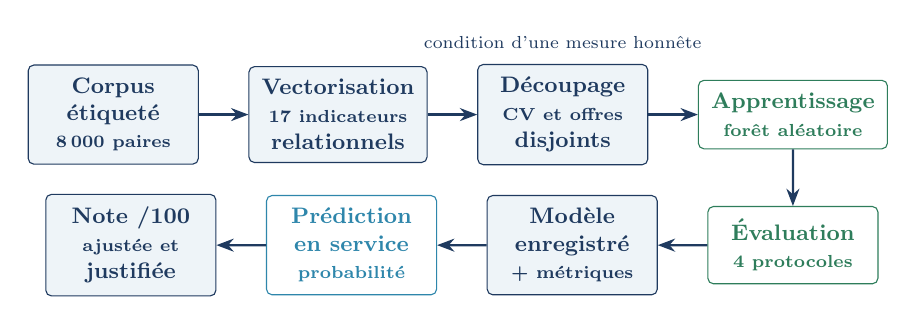
\begin{tikzpicture}[node distance=5mm and 7mm, scale=0.9, transform shape]
    \node[bloc] (corpus) {Corpus\\ étiqueté\\ \scriptsize 8\,000 paires};
    \node[bloc, right=of corpus] (vect) {Vectorisation\\ \scriptsize 17 indicateurs\\ relationnels};
    \node[bloc, right=of vect] (decoupe) {Découpage\\ \scriptsize CV et offres\\ disjoints};
    \node[blocneuf, right=of decoupe] (appr) {Apprentissage\\ \scriptsize forêt aléatoire};
    \node[blocneuf, below=8mm of appr] (eval) {Évaluation\\ \scriptsize 4 protocoles};
    \node[bloc, left=of eval] (modele) {Modèle\\ enregistré\\ \scriptsize + métriques};
    \node[blocia, left=of modele] (prod) {Prédiction\\ en service\\ \scriptsize probabilité};
    \node[bloc, left=of prod] (score) {Note /100\\ \scriptsize ajustée et\\ justifiée};

    \draw[fleche] (corpus) -- (vect);
    \draw[fleche] (vect) -- (decoupe);
    \draw[fleche] (decoupe) -- (appr);
    \draw[fleche] (appr) -- (eval);
    \draw[fleche] (eval) -- (modele);
    \draw[fleche] (modele) -- (prod);
    \draw[fleche] (prod) -- (score);

    \node[etiquette, above=1mm of decoupe] {condition d'une mesure honnête};
  \end{tikzpicture}
  \caption{De la donnée étiquetée à la note affichée au recruteur. La vectorisation est assurée par le même module à l'apprentissage et en service : c'est la condition pour que le modèle observe exactement la même chose dans les deux situations.}
  \label{fig:chaine-ml}
\end{figure}

% =====================================================================
\section{Protocole d'évaluation}
% =====================================================================

\subsection{Pourquoi quatre protocoles}
Une même performance peut être élogieuse ou trompeuse selon la manière dont on sépare les données d'apprentissage et de test. Quatre protocoles ont donc été appliqués, du plus permissif au plus exigeant, afin de mesurer l'écart entre ce qu'un protocole complaisant laisse croire et ce qu'un protocole rigoureux établit.

\begin{center}
\small
\begin{tabular}{clp{7.6cm}}
  \toprule
  \textbf{N\textsuperscript{o}} & \textbf{Protocole} & \textbf{Ce qu'il mesure} \\
  \midrule
  1 & Découpage d'origine & Traiter une offre nouvelle avec des profils déjà rencontrés \\[1mm]
  2 & Découpage par CV & Traiter un candidat inconnu sur des offres déjà connues \\[1mm]
  3 & \textbf{Découpage strict} & Traiter un candidat inconnu sur une offre nouvellement publiée --- situation réelle de la plateforme \\[1mm]
  4 & Validation française & Vérifier que le transfert d'une langue à l'autre opère \\
  \bottomrule
\end{tabular}
\end{center}

\subsection{Le découpage strict}
Le protocole~3 est celui qui fonde le chiffre retenu. Il exige que ni le curriculum vitæ ni l'offre du jeu de test n'aient été rencontrés à l'apprentissage. Cette double condition réduit fortement le volume exploitable — les paires dont un seul des deux éléments est connu sont écartées — mais elle seule reproduit la situation d'exploitation.

\begin{figure}[H]
  \centering
  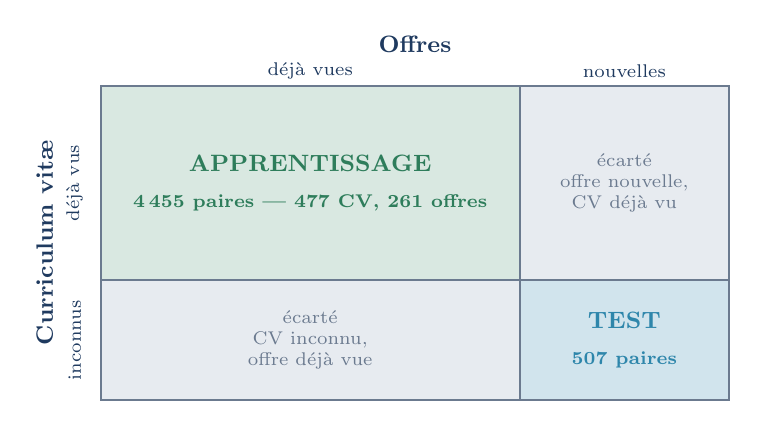
\begin{tikzpicture}[scale=0.95, transform shape]
    % Grille
    \fill[vert!18] (0,0) rectangle (5.6,2.6);
    \fill[grisclair!45] (5.6,0) rectangle (8.4,2.6);
    \fill[grisclair!45] (0,-1.6) rectangle (5.6,0);
    \fill[accent!22] (5.6,-1.6) rectangle (8.4,0);
    \draw[gris, thick] (0,-1.6) rectangle (8.4,2.6);
    \draw[gris, thick] (5.6,-1.6) -- (5.6,2.6);
    \draw[gris, thick] (0,0) -- (8.4,0);

    % Libelles
    \node[font=\small\bfseries, color=vert, align=center] at (2.8,1.3)
      {APPRENTISSAGE\\[1mm] \scriptsize 4\,455 paires --- 477 CV, 261 offres};
    \node[font=\small\bfseries, color=accent, align=center] at (7.0,-0.8)
      {TEST\\[1mm] \scriptsize 507 paires};
    \node[font=\scriptsize, color=gris, align=center] at (7.0,1.3) {écarté\\ \scriptsize offre nouvelle,\\ CV déjà vu};
    \node[font=\scriptsize, color=gris, align=center] at (2.8,-0.8) {écarté\\ \scriptsize CV inconnu,\\ offre déjà vue};

    % Axes
    \node[font=\small\bfseries, color=primaire, rotate=90] at (-0.75,0.5) {Curriculum vitæ};
    \node[font=\scriptsize, color=primaire, rotate=90] at (-0.35,1.3) {déjà vus};
    \node[font=\scriptsize, color=primaire, rotate=90] at (-0.35,-0.8) {inconnus};
    \node[font=\small\bfseries, color=primaire] at (4.2,3.15) {Offres};
    \node[font=\scriptsize, color=primaire] at (2.8,2.8) {déjà vues};
    \node[font=\scriptsize, color=primaire] at (7.0,2.8) {nouvelles};
  \end{tikzpicture}
  \caption{Découpage strict. Seules les paires dont \emph{les deux} éléments sont inconnus constituent le jeu de test. Les deux quadrants gris sont écartés : les y inclure reviendrait à évaluer le modèle sur des documents qu'il a déjà mémorisés.}
  \label{fig:decoupage}
\end{figure}

\subsection{Deux erreurs de mesure détectées}

\subsubsection{Une fuite de données dans le découpage fourni}
Le corpus était livré avec une séparation apprentissage/test préétablie. Un contrôle a révélé que cette séparation portait sur les offres uniquement : \textbf{476 des 477 curriculum vitæ du jeu de test figuraient également dans le jeu d'apprentissage}. Toute performance mesurée sur ce découpage récompense donc en partie la mémorisation des documents plutôt que la capacité à juger.

Ce constat n'invalide pas le corpus : il invalide le découpage. D'où la construction des protocoles~2 et~3.

\subsubsection{Un indicateur parasite}
Une première version des indicateurs incluait la longueur du curriculum vitæ et celle de l'offre. Ces deux mesures ressortaient parmi les plus contributives, ce qui a mis la puce à l'oreille : la longueur d'une annonce ne dit rien de l'adéquation d'un candidat, mais elle identifie l'annonce. Le modèle avait trouvé un raccourci — reconnaître l'offre plutôt que d'évaluer le profil.

Les deux indicateurs ont été supprimés. Le principe énoncé plus haut, selon lequel tout indicateur doit être relationnel, découle directement de cette observation.

\subsection{Une question mal posée}
Le corpus distingue trois niveaux : profil convenable, profil pouvant convenir, profil ne convenant pas. Sous protocole strict, le modèle n'apportait sur cette formulation \textbf{aucun gain mesurable} : $+0{,}4$~point d'exactitude sur la référence, c'est-à-dire rien.

Plutôt que d'accepter ce résultat ou de le maquiller, six configurations ont été comparées afin d'en identifier la cause.

\begin{center}
\small
\begin{tabular}{lccc}
  \toprule
  \textbf{Configuration} & \textbf{Gain} & \textbf{Exactitude} & \textbf{F1} \\
  \midrule
  \textbf{Indicateurs --- 2 classes} & \textcolor{vert}{\textbf{+8,5 \%}} & \textbf{61,9 \%} & \textbf{0,619} \\
  Combinaison --- 2 classes & +3,9 \% & 57,4 \% & 0,571 \\
  Indicateurs --- 3 classes & +0,4 \% & 46,9 \% & 0,421 \\
  Représentation complète --- 3 classes & +0,4 \% & 46,9 \% & 0,247 \\
  Représentation complète --- 2 classes & \textcolor{gris}{--0,6 \%} & 52,9 \% & 0,525 \\
  Représentation complète --- 2 classes, modèle linéaire & \textcolor{gris}{--2,2 \%} & 51,3 \% & 0,509 \\
  \bottomrule
\end{tabular}
\end{center}

\vspace{2mm}
\noindent Deux enseignements en découlent.

\textbf{La distinction entre « convient » et « pourrait convenir » n'est pas apprenable ici.} Elle relève d'une appréciation subjective que six cent quarante-trois curriculum vitæ ne suffisent pas à faire saisir. Ramenée à deux classes, la frontière devient nette et le modèle apprend.

\textbf{La représentation complète des documents échoue.} Remplacer les dix-sept indicateurs par la représentation vectorielle intégrale des deux textes — plus de quinze cents dimensions — dégrade les résultats au lieu de les améliorer. Le corpus est trop petit relativement à cette dimension : le modèle y trouve des régularités qui n'existent que dans les exemples d'apprentissage. Les dix-sept indicateurs, en concentrant l'information utile, protègent de cet écueil.

La formulation binaire a donc été retenue : \textbf{le profil convient, ou il ne convient pas}.

% =====================================================================
\section{Résultats}
% =====================================================================

\subsection{Performances par protocole}

\begin{center}
\small
\begin{tabular}{lccccc}
  \toprule
  \textbf{Protocole} & \textbf{Exactitude} & \textbf{Référence} & \textbf{Gain} & \textbf{F1} & \textbf{AUC} \\
  \midrule
  1 --- Découpage d'origine & 59,8 \% & 51,3 \% & +8,5 \% & 0,614 & 0,629 \\
  2 --- Découpage par CV & 65,4 \% & 51,8 \% & +13,6 \% & 0,664 & 0,693 \\
  \textbf{3 --- Découpage strict} & \textbf{61,9 \%} & \textbf{53,4 \%} & \textcolor{vert}{\textbf{+8,5 \%}} & \textbf{0,627} & \textbf{0,653} \\
  4 --- Validation française & 79,2 \% & 66,7 \% & +12,5 \% & 0,762 & 0,938 \\
  \bottomrule
\end{tabular}
\end{center}

\vspace{3mm}
\begin{figure}[H]
  \centering
  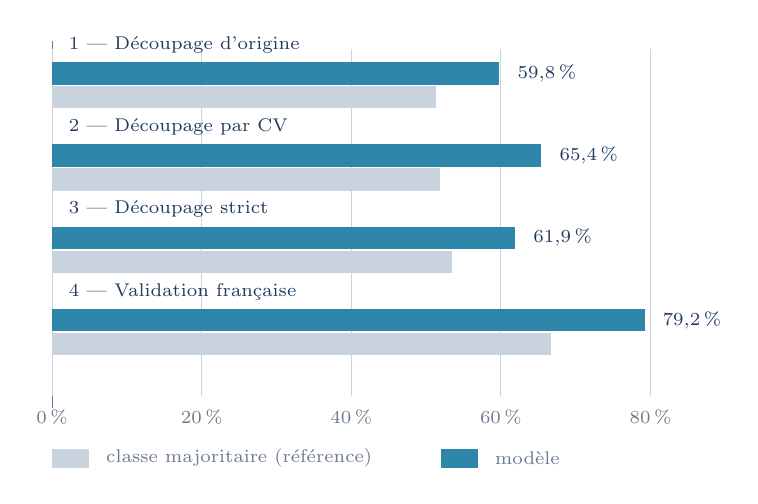
\begin{tikzpicture}[scale=0.95, transform shape]
    % Axe
    \draw[gris] (0,-0.3) -- (0,4.6);
    \foreach \x/\lab in {0/0, 2/20, 4/40, 6/60, 8/80} {
      \draw[grisclair] (\x,-0.15) -- (\x,4.5);
      \node[font=\scriptsize, color=gris, below] at (\x,-0.2) {\lab\,\%};
    }
    % Barres : y, reference, exactitude, libelle
    \foreach \y/\r/\e/\lab in {
      3.7/5.13/5.98/{1 --- Découpage d'origine},
      2.6/5.18/6.54/{2 --- Découpage par CV},
      1.5/5.34/6.19/{3 --- Découpage strict},
      0.4/6.67/7.92/{4 --- Validation française}} {
      \fill[grisclair] (0,\y) rectangle (\r,\y+0.3);
      \fill[accent] (0,\y+0.32) rectangle (\e,\y+0.62);
      \node[font=\scriptsize, color=primaire, right] at (\e+0.12,\y+0.47) {\pgfmathparse{\e*10}\pgfmathprintnumber[fixed, fixed zerofill, precision=1, use comma]{\pgfmathresult}\,\%};
      \node[font=\scriptsize, color=primaire, above right] at (0.1,\y+0.62) {\lab};
    }
    % Legende
    \fill[grisclair] (0,-1.1) rectangle (0.5,-0.85);
    \node[font=\scriptsize, color=gris, right] at (0.6,-0.97) {classe majoritaire (référence)};
    \fill[accent] (5.2,-1.1) rectangle (5.7,-0.85);
    \node[font=\scriptsize, color=gris, right] at (5.8,-0.97) {modèle};
  \end{tikzpicture}
  \caption{Exactitude du modèle comparée à la référence, protocole par protocole. L'écart entre les deux barres est la seule quantité qui compte : une exactitude élevée sur des classes déséquilibrées ne prouve rien.}
  \label{fig:resultats}
\end{figure}

\subsection{Lecture des résultats}
Le protocole~3 est celui qui doit être retenu : \textbf{61,9~\% d'exactitude contre 53,4~\% pour la référence, soit un gain de 8,5~points}, avec un F1 de 0,627 et une aire sous la courbe ROC de 0,653. C'est un résultat modeste, mais mesuré dans les conditions les plus défavorables et les plus fidèles à l'usage réel.

Le protocole~2 affiche un gain supérieur (+13,6~points) parce qu'il autorise le modèle à retrouver au test des offres déjà rencontrées. L'écart entre les protocoles~2 et~3 — cinq points — chiffre précisément ce qu'un protocole permissif fait gagner artificiellement.

Le protocole~4 mérite une réserve explicite. Ses 79,2~\% d'exactitude et son AUC de 0,938 portent sur \textbf{vingt-quatre appariements seulement}. Ce protocole établit que le transfert d'une langue à l'autre opère — un modèle appris sur des documents anglais reste utilisable sur des curriculum vitæ français — mais il ne constitue pas une mesure de précision, et il ne sera pas présenté comme telle.

\subsection{Ce sur quoi le modèle fonde son jugement}

\begin{figure}[H]
  \centering
  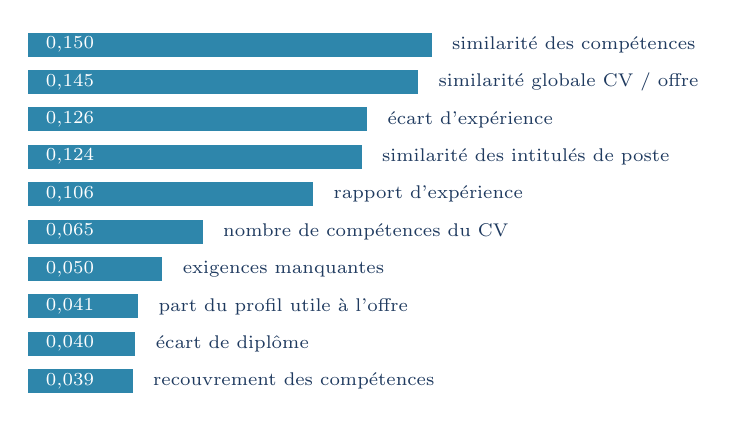
\begin{tikzpicture}[scale=0.95, transform shape]
    \foreach \y/\v/\lab in {
      4.5/0.150/{similarité des compétences},
      4.0/0.145/{similarité globale CV / offre},
      3.5/0.126/{écart d'expérience},
      3.0/0.124/{similarité des intitulés de poste},
      2.5/0.106/{rapport d'expérience},
      2.0/0.065/{nombre de compétences du CV},
      1.5/0.050/{exigences manquantes},
      1.0/0.041/{part du profil utile à l'offre},
      0.5/0.040/{écart de diplôme},
      0.0/0.039/{recouvrement des compétences}} {
      \fill[accent] (0,\y) rectangle (\v*36,\y+0.32);
      \node[font=\scriptsize, color=primaire, right] at (\v*36+0.15,\y+0.16) {\lab};
      \node[font=\scriptsize, color=white, right] at (0.12,\y+0.16) {\pgfmathprintnumber[fixed, fixed zerofill, precision=3, use comma]{\v}};
    }
  \end{tikzpicture}
  \caption{Contribution des dix indicateurs les plus déterminants. Tous décrivent une relation entre le profil et l'exigence : aucun ne permet au modèle d'identifier le document plutôt que d'en juger l'adéquation.}
  \label{fig:importances}
\end{figure}

\noindent Cette répartition constitue une vérification en soi. Les quatre indicateurs de tête — similarité des compétences, similarité globale, écart d'expérience, similarité des intitulés — sont exactement ceux qu'un recruteur mobiliserait. Aucun raccourci parasite ne subsiste, contrairement à la première version du dispositif.

% =====================================================================
\section{Intégration à la plateforme}
% =====================================================================

\subsection{Un ajustement, non une composante}
Le modèle aurait pu se voir attribuer une part fixe de la note, au même titre que les cinq composantes existantes. Ce choix a été écarté : un gain de 8,5~points d'exactitude ne justifie pas de lui confier vingt ou vingt-cinq points sur cent.

Le modèle applique donc un \textbf{ajustement borné à $\pm$8 points} sur la note établie par les règles. Une probabilité de 0,5 — le modèle est sans avis — laisse la note inchangée ; une probabilité de 1 ajoute huit points, une probabilité nulle en retire autant. La structure sur cent points, et donc la comparabilité des candidatures, est intégralement préservée.

\begin{center}
\small
\begin{tabular}{lcp{7.0cm}}
  \toprule
  \textbf{Composante} & \textbf{Poids} & \textbf{Origine} \\
  \midrule
  Compétences obligatoires & 35 & Référentiel métier appliqué au texte \\
  Compétences souhaitées & 10 & Idem, sans caractère bloquant \\
  Proximité sémantique & 25 & Comparaison du sens du document et de l'offre \\
  Années d'expérience & 20 & Périodes reconstituées \\
  Niveau de diplôme & 10 & Rubrique formation \\
  \midrule
  \textit{Avis du modèle appris} & \textit{$\pm$8} & \textit{Ajustement, appliqué après le calcul} \\
  \bottomrule
\end{tabular}
\end{center}

\subsection{Les règles restent souveraines}
Trois garanties encadrent l'intervention du modèle.

\begin{enumerate}[leftmargin=1.6em, nosep]
  \item \textbf{Aucun rattrapage.} Une candidature écartée par un critère éliminatoire — expérience insuffisante, diplôme insuffisant, compétence obligatoire absente — n'est jamais repêchée par le modèle. La décision repose alors sur un motif explicite, qu'aucun avis statistique ne doit pouvoir renverser.
  \item \textbf{Aucune dépendance.} Modèle absent, illisible, ou entraîné sur d'autres indicateurs : la note est calculée sans cette composante et l'analyse aboutit normalement. Le contrôle porte sur la liste exacte des indicateurs attendus, de sorte qu'un modèle périmé soit refusé plutôt qu'exploité de travers.
  \item \textbf{Aucune opacité.} La probabilité, la note avant ajustement et l'ajustement effectivement appliqué sont restitués au recruteur.
\end{enumerate}

\begin{figure}[H]
  \centering
  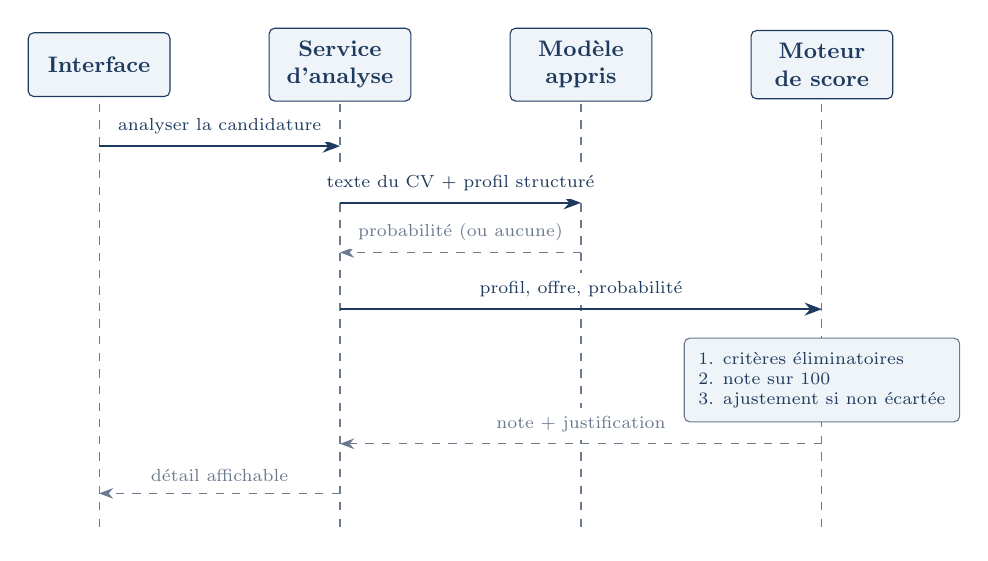
\begin{tikzpicture}[scale=0.9, transform shape,
      msg/.style={font=\scriptsize, color=primaire, fill=white, inner sep=1.2mm, align=center},
      msgret/.style={msg, text=gris}]
    % Lignes de vie
    \foreach \x/\nom in {0/{Interface}, 3.4/{Service\\ d'analyse}, 6.8/{Modèle\\ appris}, 10.2/{Moteur\\ de score}} {
      \node[bloc, minimum width=20mm] (t\x) at (\x,0) {\nom};
      \draw[gris, dashed] (\x,-0.55) -- (\x,-6.6);
    }
    % Messages
    \draw[fleche] (0,-1.15) -- node[msg, above=0.4mm] {analyser la candidature} (3.4,-1.15);
    \draw[fleche] (3.4,-1.95) -- node[msg, above=0.4mm] {texte du CV + profil structuré} (6.8,-1.95);
    \draw[flechefine, dashed] (6.8,-2.65) -- node[msgret, above=0.4mm] {probabilité (ou aucune)} (3.4,-2.65);
    \draw[fleche] (3.4,-3.45) -- node[msg, above=0.4mm] {profil, offre, probabilité} (10.2,-3.45);

    \node[draw=gris, fill=fondclair, rounded corners=2pt, font=\scriptsize, align=left,
          text=primaire, inner sep=2mm] at (10.2,-4.45)
      {1. critères éliminatoires\\ 2. note sur 100\\ 3. ajustement si non écartée};

    \draw[flechefine, dashed] (10.2,-5.35) -- node[msgret, above=0.4mm] {note + justification} (3.4,-5.35);
    \draw[flechefine, dashed] (3.4,-6.05) -- node[msgret, above=0.4mm] {détail affichable} (0,-6.05);
  \end{tikzpicture}
  \caption{Séquence d'analyse d'une candidature. Le modèle est interrogé avant le calcul, mais son avis n'est appliqué qu'après les critères éliminatoires : l'ordre garantit qu'il ne peut jamais les contourner.}
  \label{fig:sequence}
\end{figure}

\subsection{Organisation des modules}

\begin{figure}[H]
  \centering
  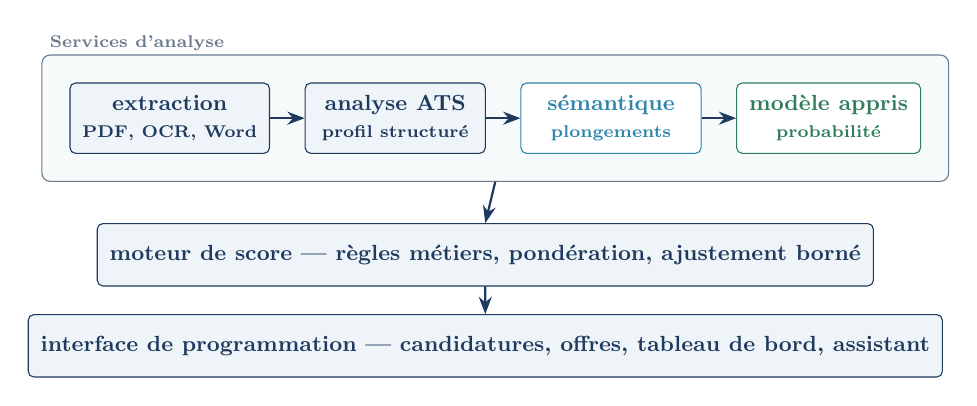
\begin{tikzpicture}[scale=0.88, transform shape, node distance=4mm and 5mm]
    \node[bloc, minimum width=26mm] (extraction) {extraction\\ \scriptsize PDF, OCR, Word};
    \node[bloc, minimum width=26mm, right=of extraction] (ats) {analyse ATS\\ \scriptsize profil structuré};
    \node[blocia, minimum width=26mm, right=of ats] (sem) {sémantique\\ \scriptsize plongements};
    \node[blocneuf, minimum width=26mm, right=of sem] (ml) {modèle appris\\ \scriptsize probabilité};

    \node[bloc, minimum width=112mm, below=10mm of ats.south, anchor=north, xshift=13mm]
      (scoring) {moteur de score --- règles métiers, pondération, ajustement borné};
    \node[bloc, minimum width=112mm, below=4mm of scoring] (api)
      {interface de programmation --- candidatures, offres, tableau de bord, assistant};

    \begin{scope}[on background layer]
      \node[draw=gris, rounded corners=3pt, fill=fondclair!50, inner sep=3.5mm,
            fit=(extraction)(ml)] (services) {};
    \end{scope}
    \node[font=\scriptsize\bfseries, color=gris, above=1.6mm of services.north west, anchor=west]
      {Services d'analyse};

    \draw[fleche] (extraction) -- (ats);
    \draw[fleche] (ats) -- (sem);
    \draw[fleche] (sem) -- (ml);
    \draw[fleche] (services.south) -- (scoring.north);
    \draw[fleche] (scoring) -- (api);
  \end{tikzpicture}
  \caption{Place du nouveau module dans l'architecture. Il s'insère en fin de chaîne d'analyse et alimente le moteur de score, sans modification des modules existants.}
  \label{fig:composants}
\end{figure}

\subsection{Restitution au recruteur}
L'exigence d'explicabilité, centrale depuis le début du projet, s'applique au modèle comme au reste. Le panneau de détail d'une candidature affiche désormais, sous les cinq composantes du calcul, la probabilité estimée, la note obtenue par les seules règles et l'ajustement appliqué.

\begin{lstlisting}[caption={L'ajustement n'est calculé que si aucun critère éliminatoire n'est déclenché.}]
ajustement = 0.0
if probabilite_modele is not None and not eliminatoires:
    ajustement = (probabilite_modele - 0.5) * 2 * AMPLITUDE_MODELE

score = round(score_regles + ajustement)
if eliminatoires:
    score = min(score, 45)   # ecarte par regle metier
\end{lstlisting}

\begin{figure}[H]
  \centering
  \IfFileExists{captures/15_avis_modele_detail.jpg}{%
    \fbox{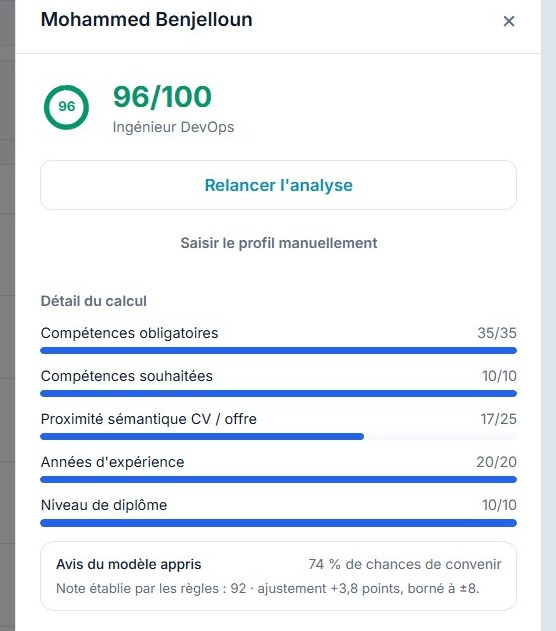
\includegraphics[width=0.56\textwidth]{captures/15_avis_modele_detail}}%
  }{%
    \fbox{\parbox[c][5cm][c]{0.56\textwidth}{\centering\color{gris}%
      Capture manquante : \texttt{\detokenize{captures/15_avis_modele_detail.jpg}}}}%
  }
  \caption{Détail d'une note, tel que présenté au recruteur. Sous les cinq composantes du calcul
  figure l'avis du modèle : probabilité que le profil convienne, note établie par les règles et
  ajustement effectivement appliqué avec sa borne. La note affichée, 96, est la somme vérifiable
  de 92 et de 3,8.}
  \label{fig:avismodele}
\end{figure}

% =====================================================================
\section{Consolidation de la sécurité applicative}\label{sec:consolidation}
% =====================================================================

\subsection{Origine de ces travaux}
L'intégration du modèle achevée, une relecture systématique du code a été menée avant la clôture du stage, en prenant délibérément le point de vue d'un utilisateur mal intentionné plutôt que celui du développeur. Cette relecture a mis au jour un défaut réel, qui ne relevait ni d'une fonction manquante ni d'un défaut d'affichage, et dont la portée justifie qu'il soit exposé ici en toute franchise.

\subsection{Un cloisonnement incomplet entre recruteurs}

\subsubsection{Le défaut}
Le contrôle d'accès par rôles répond à la question « cet utilisateur a-t-il le droit de consulter des candidatures ? ». Il ne répond pas à « celle-ci ? ». Or deux recruteurs détiennent exactement les mêmes permissions ; ce qui les sépare n'est pas le rôle mais le \textbf{périmètre} : la chaîne de propriété qui va du recruteur à son offre, de l'offre à ses candidatures, et de la candidature au document déposé.

Plusieurs routes vérifiaient la permission sans vérifier le périmètre. Un recruteur authentifié pouvait ainsi, en modifiant l'identifiant dans l'adresse d'une requête, consulter le détail d'une candidature adressée à une entreprise concurrente, et télécharger le curriculum vitæ correspondant. Aucune interface n'y conduisait, mais l'interface n'est pas une frontière de sécurité.

\subsubsection{La correction}
La vérification de propriété a été centralisée dans un module dédié, plutôt que réécrite à chaque route. Un contrôle dispersé se maintient mal : il suffit d'un point d'accès ajouté plus tard pour rouvrir la brèche, et rien dans le code ne signale l'oubli.

\begin{lstlisting}[caption={Résolution d'une ressource avec vérification du périmètre. La fonction rend un couple : la ressource si l'accès est légitime, sinon la réponse de refus déjà formée.}]
def candidature(utilisateur, identifiant):
    obj = Application.query.get(identifiant)
    if obj is None:
        return None, (jsonify(error="Candidature introuvable."), 404)
    if not possede_offre(utilisateur, obj.offer):
        return None, (jsonify(error=MESSAGE_PERIMETRE), 403)
    return obj, None
\end{lstlisting}

\noindent Les listes suivent le même principe : la requête est restreinte au périmètre avant d'être exécutée, et non filtrée après coup.

\subsubsection{La vérification}
Onze cas de test ont été écrits \textbf{du point de vue de l'attaquant} : le recruteur~B demande explicitement une ressource du recruteur~A et doit se voir opposer un refus. Cette formulation n'est pas indifférente. Un test qui se contenterait de vérifier que~A consulte bien ses propres données passerait tout aussi bien \emph{sans} le correctif, et n'aurait donc aucune valeur probante.

\subsection{Verrou de connexion}
Le formulaire de connexion n'opposait aucune limite au nombre d'essais. Un verrou temporaire a été ajouté après une série d'échecs consécutifs, avec deux précautions.

La première : le verrou est évalué \textbf{avant} la vérification du mot de passe. Un contrôle placé après aurait laissé subsister un moyen de distinguer un compte verrouillé d'un compte inexistant, à la simple mesure du temps de réponse.

La seconde : la réponse annonce la durée restante. Un refus muet conduit l'utilisateur légitime --- qui s'est simplement trompé --- à multiplier les tentatives et à prolonger son propre verrou, quand il devrait seulement patienter.

\subsection{Séparation des domaines de l'assistant}
L'assistant conversationnel avait été conçu pour le recruteur. Son ouverture à l'administrateur, souhaitée en cours de sprint, posait une difficulté qui n'était pas d'interface : la base de connaissances interrogée contenait le contenu des candidatures, et le rôle administrateur ne détient pas le droit de les consulter. Une conversation ne doit pas devenir le moyen de contourner le modèle de permissions.

Deux bases de connaissances \textbf{disjointes} ont donc été constituées, l'une pour le recrutement et l'autre pour l'administration --- comptes en attente, signalements ouverts, activité récente, aide à l'usage. Un test vérifie qu'aucun document du domaine administration n'est de nature « candidature » ou « offre », et qu'aucune note d'adéquation n'y figure.

% =====================================================================
\section{Restitution et orientation}\label{sec:restitution}
% =====================================================================

\subsection{Le pilotage rendu à l'application}
La restitution décisionnelle était prévue sous la seule forme de rapports Power BI. Ce choix a été complété plutôt que remplacé : un recruteur qui doit ouvrir un outil séparé pour savoir où en sont ses recrutements ne le fait pas. Un écran d'analyse a donc été intégré à la plateforme, alimenté par les mêmes données.

Il présente la répartition des notes, les motifs d'écartement regroupés par nature, les compétences les plus souvent absentes des dossiers reçus, et le délai médian avant première décision. Ce dernier indicateur mérite une note de méthode : la candidature ne porte pas de date de modification, et le délai est donc lu dans le \textbf{journal d'audit}, à la première trace de changement de statut. Le journal, conçu comme une garantie de traçabilité, acquiert ainsi une seconde utilité.

\subsubsection{La section qui engage le système}
L'écran comporte une section intitulée « le classement tient-il ses promesses ? », qui confronte la note calculée \emph{avant} l'entretien au verdict porté \emph{après}, sur les candidats réellement reçus. Deux quantités y sont comptées séparément, et cette séparation est délibérée : les \textbf{faux espoirs} --- bien notés, mal évalués en entretien --- et les \textbf{pépites manquées} --- mal notées, bien évaluées. Les confondre en un taux d'erreur unique masquerait que leurs coûts n'ont rien de comparable. Un faux espoir coûte une heure d'entretien ; une pépite manquée coûte un candidat, définitivement.

\subsection{L'orientation du candidat}
Le candidat n'avait, jusqu'ici, qu'un catalogue à parcourir. Il postulait au jugé, et le recruteur recevait des dossiers hors sujet : les deux y perdaient.

Le moteur a été retourné. Le calcul qui répond « ce candidat convient-il à cette offre ? » répond désormais aussi « quelles offres conviennent à ce profil ? », sans qu'aucune logique de notation ait été réimplémentée. Le candidat déclare ses compétences, son expérience et son diplôme ; les offres lui sont présentées par proximité décroissante. Lorsqu'un curriculum vitæ a déjà été analysé, le profil qui en est extrait \textbf{prime sur le profil déclaré} : l'observé l'emporte sur le déclaré, personne ne vérifiant une saisie.

\medskip
\noindent\textbf{Aucune note n'est communiquée au candidat, et c'est une règle et non un oubli.} Un chiffre sans son barème invite au malentendu, et une personne qui aurait lu « 87~\% » avant d'être écartée disposerait d'un grief légitime. Ce qui lui est montré, ce sont les \textbf{compétences manquantes} --- la seule chose qu'elle puisse corriger --- et un niveau de correspondance qualitatif. Un test vérifie qu'aucune valeur numérique d'adéquation ne figure dans la réponse, ni au premier niveau ni dans un sous-objet.

\subsection{Première connexion et retenue des animations}
Une visite guidée se déclenche à la première connexion, dans une version propre à chaque rôle : les trois profils n'entrent pas par la même porte, et une visite unique les servirait tous mal. Elle désigne les éléments par des attributs nommés plutôt que par des classes de style --- une classe change au premier ajustement visuel et casse la visite en silence.

Les transitions ajoutées à l'interface obéissent à une contrainte simple : elles accompagnent une information, jamais l'inverse. Un compteur qui s'incrémente donne l'ordre de grandeur avant le chiffre exact ; une jauge qui se remplit rend la proportion lisible sans la lire. Toutes sont désactivées d'un seul bloc lorsque le système de l'utilisateur signale une préférence pour un mouvement réduit, réglage qui répond à des troubles vestibulaires réels et n'est pas une question de goût.

% =====================================================================
\section{Industrialisation et exploitation}\label{sec:industrialisation}
% =====================================================================

\subsection{La chaîne d'intégration et de livraison}
La chaîne d'intégration continue comptait deux travaux ; elle en compte \textbf{sept}, exécutés à chaque poussée de code.

\begin{center}
\small
\begin{tabular}{lp{8.6cm}}
  \toprule
  \textbf{Travail} & \textbf{Objet} \\
  \midrule
  Service applicatif & Analyse statique et exécution de la totalité des tests \\[1mm]
  Interface & Analyse statique et construction de production \\[1mm]
  Dépendances & Recherche de vulnérabilités connues dans les bibliothèques des deux écosystèmes \\[1mm]
  Sécurité du dépôt & Analyse Trivy : secrets exposés, défauts de configuration \\[1mm]
  Sécurité du code & Analyse statique orientée sûreté (Bandit, Semgrep) sur les deux écosystèmes \\[1mm]
  Images & Construction des deux images, analyse de leur contenu, publication au registre avec inventaire logiciel \\[1mm]
  Assemblage & Démarrage de la pile complète et interrogation des sondes de disponibilité \\
  \bottomrule
\end{tabular}
\end{center}

\vspace{2mm}
\noindent\textbf{Une précision sur l'analyse statique de sûreté.} \texttt{flake8} et
ESLint étaient présents depuis le premier sprint, mais ils jugent le style et
non la sûreté : ils n'ont aucune opinion sur un hachage affaibli ou sur une
requête construite par concaténation. Le travail ajouté comble cette lacune.

Sa mise en service illustre ce qu'on attend d'un tel outil. Douze constats ont
été relevés au premier passage. \textbf{Cinq ont donné lieu à une correction} :
un condensat MD5 servant de clé de cache désormais déclaré comme non
cryptographique, le mot de passe initial de l'administrateur lu depuis
l'environnement, et surtout la vérification du schéma de l'adresse du modèle de
langue avant tout appel réseau --- sans elle, une adresse en \texttt{file://}
aurait transformé un appel distant en lecture de fichier local. \textbf{Les sept
autres sont des faux positifs}, chacun accompagné dans le code du motif qui
l'écarte : des libellés français pris pour des mots de passe, un générateur
pseudo-aléatoire employé pour composer un jeu de démonstration, et des noms de
vues provenant d'une constante du module et non d'une saisie.

Le rapport d'un analyseur n'a de valeur que lu et arbitré. Le laisser produire
des avertissements que personne ne tranche revient à ne pas l'avoir.

\medskip
\noindent Le dernier travail est celui qui apporte le plus. Les cinq premiers vérifient des composants isolément ; celui-ci vérifie qu'ils \textbf{fonctionnent ensemble} --- une base de données qui se lève, un service qui applique ses migrations et répond, une interface qui se construit avec la bonne adresse d'interface de programmation. C'est l'assemblage, non les composants, qui échoue en pratique.

\subsection{Chaîne d'approvisionnement logicielle}
Chaque construction produit un \textbf{inventaire des composants} de l'image, publié comme artefact. La justification est directe : lorsqu'une vulnérabilité est rendue publique, la question n'est pas de savoir si elle est grave --- l'avis le dit --- mais si le projet en est porteur. Sans inventaire, y répondre demande une inspection manuelle ; avec, c'est une recherche.

Les images sont étiquetées par l'empreinte du commit qui les a produites. Chaque état du code correspond donc à un artefact déployable et identifiable, ce qui rend le retour arrière trivial : redémarrer avec l'étiquette précédente.

Une veille automatique propose enfin les montées de version des dépendances. Elle est configurée pour \textbf{ignorer les montées de version majeures}, qui appellent une lecture des notes de version et non une acceptation automatique, et pour viser la branche de développement plutôt que la branche principale.

\subsection{Observabilité}
Trois dispositifs ont été ajoutés à la chaîne d'analyse.

\begin{itemize}[leftmargin=1.5em, itemsep=2pt]
  \item \textbf{Chronométrage par étape.} Le coût d'une analyse se répartit très inégalement --- la reconnaissance optique et le calcul des plongements dominent --- et seule la mesure permet de savoir laquelle ralentit une analyse donnée. Les durées sont conservées avec le résultat.
  \item \textbf{Bloc de provenance.} Chaque note porte la version du moteur, les modèles utilisés, l'empreinte du code et la date d'analyse. Une note contestée six mois plus tard doit pouvoir être rattachée à la version exacte qui l'a produite ; sans cela, la reproduire est une conjecture.
  \item \textbf{Identifiant de requête et sondes distinctes.} Une sonde de \emph{vivacité} répond tant que le service est en vie ; une sonde de \emph{disponibilité} n'annonce l'état favorable que si la base de données et les modèles répondent. Les confondre conduit un orchestrateur à envoyer du trafic vers un service incapable de le traiter.
\end{itemize}

\subsection{Ce que la conteneurisation apporte, et ce qu'elle n'apporte pas}
La plateforme se lève d'une seule commande, sur n'importe quel poste, sans installation préalable d'un interpréteur, d'une base de données ni d'un environnement d'exécution. C'est ce qui rend la chaîne d'intégration crédible : elle exécute la même image que le poste de développement, et un échec y est reproductible localement.

\medskip
\noindent\textbf{Il convient en revanche de ne pas confondre livraison et déploiement.} Le projet dispose d'une \emph{livraison} continue : chaque commit produit un artefact prêt à être déployé. Il ne dispose pas de \emph{déploiement} continu : aucun serveur ne reçoit cet artefact. La procédure de déploiement est écrite et versionnée, mais désactivée faute d'infrastructure dans le cadre du stage. La distinction est nette et un jury la connaît ; la revendiquer serait une faute.

% =====================================================================
\section{Vérification}
% =====================================================================
La couverture de tests a été portée de soixante-neuf à \textbf{cent quatre-vingt-douze} cas réussis, auxquels s'ajoutent deux cas ignorés lorsque les modèles optionnels ne sont pas présents.

\begin{center}
\small
\begin{tabular}{lcc}
  \toprule
  \textbf{Domaine testé} & \textbf{Cas} & \textbf{Résultat} \\
  \midrule
  Authentification et sessions & 6 & \textcolor{vert}{Réussis} \\
  \textbf{Verrou de connexion} & \textbf{5} & \textcolor{vert}{Réussis} \\
  Contrôle d'accès par permissions & 3 & \textcolor{vert}{Réussis} \\
  \textbf{Cloisonnement par périmètre} & \textbf{11} & \textcolor{vert}{Réussis} \\
  Moteur de notation et règle de présélection & 14 & \textcolor{vert}{Réussis} \\
  Modèle appris --- robustesse et bornes & 5 & \textcolor{vert}{Réussis} \\
  Chaîne d'analyse d'un curriculum vitæ & 14 & \textcolor{vert}{Réussis} \\
  Reconstitution du profil structuré & 16 & \textcolor{vert}{Réussis} \\
  Contrôles d'anomalies sur les dossiers & 22 & \textcolor{vert}{Réussis} \\
  Assistant --- domaine recrutement & 20 & \textcolor{vert}{Réussis} \\
  \textbf{Assistant --- domaine administration} & \textbf{11} & \textcolor{vert}{Réussis} \\
  \textbf{Orientation du candidat} & \textbf{10} & \textcolor{vert}{Réussis} \\
  \textbf{Analyse décisionnelle} & \textbf{8} & \textcolor{vert}{Réussis} \\
  \textbf{Observabilité et provenance} & \textbf{9} & \textcolor{vert}{Réussis} \\
  \textbf{Document manquant et réparation} & \textbf{4} & \textcolor{vert}{Réussis} \\
  Qualification des recruteurs & 12 & \textcolor{vert}{Réussis} \\
  Validation des comptes et corbeille & 14 & \textcolor{vert}{Réussis} \\
  Offres, notifications, profil & 10 & \textcolor{vert}{Réussis} \\
  \midrule
  \textbf{Total collecté} & \textbf{194} & \textcolor{vert}{\textbf{192 réussis, 2 ignorés}} \\
  \bottomrule
\end{tabular}
\end{center}

\vspace{1mm}
\noindent Les deux cas ignorés dépendent de modèles optionnels absents de l'environnement d'intégration ; ils sont exécutés localement lorsque ces modèles sont présents. Aucun cas n'est en échec.

\vspace{2mm}
\noindent Trois familles de cas méritent d'être distinguées, parce qu'elles ne testent pas un comportement mais un \textbf{engagement}.

\medskip
\noindent\textbf{Le cloisonnement} (11 cas). Chacun est écrit du point de vue de l'attaquant : le recruteur~B réclame nommément une ressource du recruteur~A. Une formulation inverse aurait produit des tests qui passent avec ou sans le correctif.

\medskip
\noindent\textbf{Le silence de la note vis-à-vis du candidat} (dans les 10 cas d'orientation). Un cas énumère les clés interdites --- note, score, détail du calcul, probabilité --- et vérifie leur absence à chaque niveau d'imbrication de la réponse. L'engagement porte sur ce qui ne doit \emph{pas} être transmis, et un test de présence ne l'aurait pas couvert.

\medskip
\noindent\textbf{La robustesse du modèle} (5 cas). L'exigence testée n'est pas la qualité des prédictions --- elle relève des protocoles d'évaluation --- mais la garantie qu'\textbf{aucune analyse ne peut échouer à cause du modèle} : fichier absent, fichier corrompu, modèle entraîné sur d'autres indicateurs. Chacun doit aboutir à une note calculée sans cette composante. S'y ajoutent la neutralité à probabilité~0,5, le respect de la borne de $\pm$8~points, et l'impossibilité de rattraper une candidature écartée par une règle.

% =====================================================================
\section{Ce qui n'a pas été fait}\label{sec:perspectives}
% =====================================================================
Un rapport de clôture qui ne présenterait que des réussites serait suspect. Deux éléments du périmètre élargi n'ont pas été livrés, et deux autres ont été livrés sous une forme réduite. Ils sont exposés ici avec leur motif, et non renvoyés à une rubrique de perspectives.

\subsection{Déploiement sur un serveur}
La procédure de déploiement est écrite, versionnée et paramétrée, mais \textbf{désactivée} : elle ne s'exécute qu'en présence des identifiants d'un serveur cible, absents du dépôt. Aucune infrastructure n'a été mise à disposition dans le cadre du stage, et aucun service payant n'a été souscrit --- contrainte assumée dès le début du projet.

La conséquence doit être énoncée clairement : la plateforme dispose d'une \emph{livraison} continue, non d'un \emph{déploiement} continu. Ce qui manque n'est pas du code mais une machine.

\subsection{Tests de bout en bout}
Les parcours des trois profils sont vérifiés manuellement et documentés par un script d'enregistrement, mais ils ne sont pas automatisés en navigateur. L'arbitrage a été explicite : à temps égal, onze cas de cloisonnement écrits du point de vue de l'attaquant protègent davantage la plateforme qu'un parcours de connexion automatisé. Ce choix reste discutable, et il est présenté comme tel.

\subsection{Deux livrables réduits}
\textbf{L'audit de biais} a été conduit et son résultat est énoncé --- au plus deux points de variation, imputables à la similarité sémantique qui encode le document entier, identité comprise. Il ne s'agit pas d'une étude statistique sur un large échantillon, et la formule « sans biais » serait fausse. L'écart est négligeable mais réel.

\textbf{La métrologie d'exploitation} se limite au chronométrage conservé avec chaque analyse. Il n'existe pas de collecte centralisée ni de système d'alerte, dont l'intérêt reste théorique tant qu'aucun serveur ne reçoit de trafic.

\subsection{Récapitulatif}
\begin{center}
\small
\begin{tabular}{lcp{7.4cm}}
  \toprule
  \textbf{Élément} & \textbf{État} & \textbf{Motif} \\
  \midrule
  Déploiement sur serveur & \textcolor{ambre}{Non activé} & Absence d'infrastructure ; procédure écrite et prête \\[1mm]
  Tests de bout en bout & \textcolor{ambre}{Non réalisé} & Arbitrage en faveur des tests de sécurité \\[1mm]
  Audit de biais & \textcolor{accent}{Réduit} & Mesure conduite, portée statistique limitée \\[1mm]
  Métrologie centralisée & \textcolor{accent}{Réduite} & Sans objet en l'absence de trafic réel \\
  \bottomrule
\end{tabular}
\end{center}

% =====================================================================
\section{Planification}
% =====================================================================

\begin{figure}[H]
  \centering
  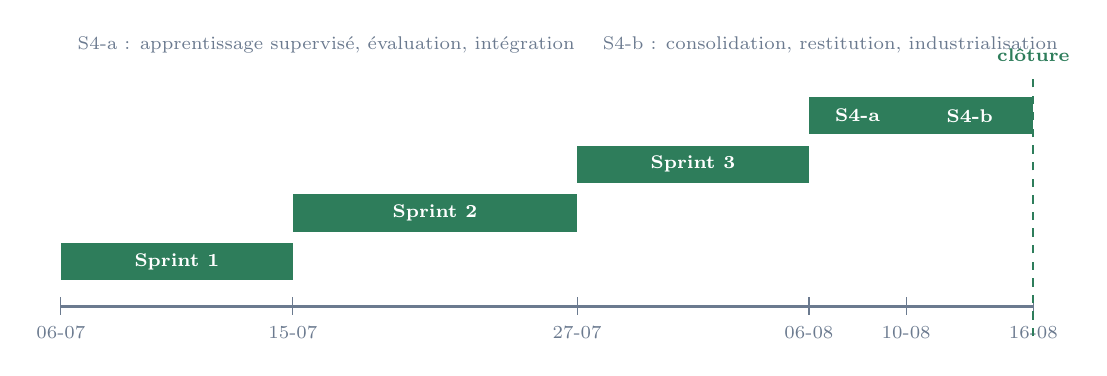
\begin{tikzpicture}[scale=0.95, transform shape]
    \draw[gris, thick] (0,0) -- (13,0);
    \foreach \x/\lab in {0/06-07, 3.1/15-07, 6.9/27-07, 10/06-08, 11.3/10-08, 13/16-08} {
      \draw[gris] (\x, 0.12) -- (\x, -0.12);
      \node[font=\scriptsize, color=gris, below] at (\x, -0.15) {\lab};
    }
    \fill[vert] (0, 0.35) rectangle (3.1, 0.85);
    \node[white, font=\scriptsize\bfseries] at (1.55, 0.6) {Sprint 1};
    \fill[vert] (3.1, 1.0) rectangle (6.9, 1.5);
    \node[white, font=\scriptsize\bfseries] at (5.0, 1.25) {Sprint 2};
    \fill[vert] (6.9, 1.65) rectangle (10, 2.15);
    \node[white, font=\scriptsize\bfseries] at (8.45, 1.9) {Sprint 3};
    \fill[vert] (10, 2.3) rectangle (11.3, 2.8);
    \node[white, font=\scriptsize\bfseries] at (10.65, 2.55) {S4-a};
    \fill[vert] (11.3, 2.3) rectangle (13, 2.8);
    \node[white, font=\scriptsize\bfseries] at (12.15, 2.55) {S4-b};
    \draw[dashed, thick, color=vert] (13, -0.4) -- (13, 3.15);
    \node[font=\scriptsize\bfseries, color=vert, above] at (13, 3.15) {clôture};
    \node[font=\scriptsize, color=gris, right] at (0.1, 3.5)
      {S4-a : apprentissage supervisé, évaluation, intégration \quad
       S4-b : consolidation, restitution, industrialisation};
  \end{tikzpicture}
  \caption{Déroulement du projet. Les quatre sprints sont achevés, la livraison finale au 16 août ayant été tenue.}
  \label{fig:gantt4}
\end{figure}

\begin{center}
\small
\begin{tabular}{lcp{7.0cm}}
  \toprule
  \textbf{Période} & \textbf{Jours} & \textbf{Contenu} \\
  \midrule
  07/08 -- 10/08 & 4 & Corpus, modèle supervisé, protocoles d'évaluation, intégration au score, tests \\[1mm]
  11/08 -- 13/08 & 3 & Relecture de sécurité, cloisonnement par périmètre, verrou de connexion, séparation des domaines de l'assistant \\[1mm]
  14/08 -- 15/08 & 2 & Analyse décisionnelle intégrée, orientation du candidat, visite guidée, observabilité \\[1mm]
  16/08 & 1 & Industrialisation de la construction et de la livraison, documentation, jeu de démonstration \\
  \bottomrule
\end{tabular}
\end{center}

% =====================================================================
\section{Risques et mesures}
% =====================================================================

\begin{center}
\small
\begin{tabular}{p{4.4cm}cp{7.6cm}}
  \toprule
  \textbf{Risque} & \textbf{Criticité} & \textbf{Mesure retenue} \\
  \midrule
  Interprétation erronée des chiffres à la soutenance & \textcolor{ambre}{\textbf{Élevée}} & Distinction explicite, dans le rapport et à l'oral, entre l'exactitude du modèle et les indicateurs du dispositif complet ; chaque chiffre est présenté avec le protocole qui l'établit. \\[1mm]
  Confusion entre livraison et déploiement continus & \textcolor{ambre}{\textbf{Élevée}} & Formulation arrêtée et répétée : intégration et livraison automatisées, déploiement prêt mais non activé. Aucune revendication au-delà. \\[1mm]
  Performance modeste du modèle & Faible & Ajustement volontairement borné à $\pm$8 points : la qualité du classement ne dépend pas du modèle, qui n'apporte qu'un départage complémentaire. \\[1mm]
  Volume restreint du jeu de validation français & Moyenne & Ce protocole est présenté comme une vérification de transfert linguistique, jamais comme une mesure de précision. \\[1mm]
  Défauts de cloisonnement réintroduits par un ajout ultérieur & Moyenne & Vérification centralisée dans un module unique plutôt que répétée par route ; onze tests écrits du point de vue de l'attaquant échouent si la vérification est omise. \\[1mm]
  Coût des services externes & Faible & Chaîne complète construite sur des outils gratuits ou en licence libre ; aucun service payant n'est requis pour l'exécution. \\
  \bottomrule
\end{tabular}
\end{center}

% =====================================================================
\section{Conclusion}
% =====================================================================
La partie du Sprint~4 consacrée à l'apprentissage supervisé est achevée. La fonction déclarée abandonnée au sprint précédent est désormais réalisée : un corpus a été identifié puis contrôlé, dix-sept indicateurs relationnels ont été définis, un modèle a été entraîné, et son apport a été mesuré sous quatre protocoles dont le plus exigeant reproduit la situation réelle de la plateforme.

Le chiffre retenu — 8,5 points d'exactitude au-dessus de la référence — est modeste, et il est présenté comme tel. Il vaut davantage que les gains supérieurs qu'auraient affichés des protocoles plus permissifs : ceux-ci mesuraient en partie la mémorisation de documents déjà vus. Deux erreurs de mesure ont d'ailleurs été détectées et corrigées en cours de route, une fuite de données dans le découpage fourni et un indicateur permettant au modèle d'identifier l'offre au lieu de la juger.

L'intégration retenue tire les conséquences de cette mesure. Le modèle n'occupe pas une part fixe de la note mais applique un ajustement borné, ne peut jamais rattraper une candidature écartée par une règle explicite, et son absence n'empêche aucune analyse d'aboutir. La plateforme conserve ainsi la propriété qui fait sa valeur : chaque note attribuée reste intégralement justifiable auprès du recruteur comme auprès du candidat.

\medskip
La seconde partie du sprint a porté sur une exigence différente, et sans doute plus déterminante pour la suite. Une relecture menée du point de vue d'un utilisateur mal intentionné a révélé que les permissions, correctement appliquées, ne suffisaient pas : elles disent ce qu'un rôle a le droit de faire, non sur quelles ressources. Le défaut a été corrigé au moyen d'une vérification centralisée et de onze tests qui échouent si elle est omise. Un projet d'école peut se contenter d'une fonction qui marche ; un produit destiné à recevoir des candidatures réelles ne le peut pas.

Les mêmes jours ont ramené le pilotage dans l'application plutôt que dans un outil séparé, retourné le moteur au bénéfice du candidat --- qui reçoit ses compétences manquantes et jamais sa note --- et industrialisé la construction : six travaux d'intégration, deux images publiées avec leur inventaire logiciel, une veille des dépendances.

\medskip
\noindent\textbf{Le projet est livré dans son périmètre fonctionnel intégral.} Ce qui manque relève de l'exploitation --- un serveur qui reçoive l'artefact, des parcours automatisés en navigateur --- et la section~\ref{sec:perspectives} l'énonce sans le déguiser en perspective. La distinction entre livraison continue, acquise, et déploiement continu, non réalisé, sera maintenue à l'oral comme elle l'est ici.

Reste, pour la soutenance, ce qu'aucun rapport ne remplace : montrer le dispositif en fonctionnement, et notamment la démonstration qui l'expose le mieux --- retirer une permission à un rôle et voir l'accès refusé à la requête suivante, sans attendre l'expiration d'aucune session.

\end{document}
